% 三条直线交于一点，6 个角，∠1=50, ∠2=60
\documentclass[tikz,border=4pt]{standalone}
\usepackage{ctex}
\usepackage{amsmath}
\usetikzlibrary{calc, arrows.meta}
\begin{document}
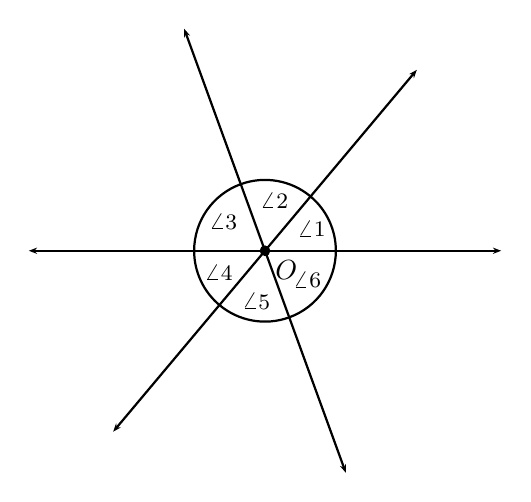
\begin{tikzpicture}[scale=1.0, thick]
  \coordinate (O) at (0,0);
  \pgfmathsetmacro{\angA}{0}
  \pgfmathsetmacro{\angB}{50}
  \pgfmathsetmacro{\angC}{110}
  \foreach \a in {\angA,\angB,\angC} {
    \draw[-{Stealth[length=3pt]}] (O) -- ({3*cos(\a)}, {3*sin(\a)});
    \draw[-{Stealth[length=3pt]}] (O) -- ({3*cos(\a+180)}, {3*sin(\a+180)});
  }
  % 标 6 个角
  \draw (0.9,0) arc (0:\angB:0.9);
  \node[font=\footnotesize] at ({0.65*cos(\angB/2)}, {0.65*sin(\angB/2)}) {$\angle 1$};
  \draw ({0.9*cos(\angB)}, {0.9*sin(\angB)}) arc (\angB:\angC:0.9);
  \node[font=\footnotesize] at ({0.65*cos((\angB+\angC)/2)}, {0.65*sin((\angB+\angC)/2)}) {$\angle 2$};
  \draw ({0.9*cos(\angC)}, {0.9*sin(\angC)}) arc (\angC:180:0.9);
  \node[font=\footnotesize] at ({0.65*cos((\angC+180)/2)}, {0.65*sin((\angC+180)/2)}) {$\angle 3$};
  \draw ({0.9*cos(180)}, 0) arc (180:180+\angB:0.9);
  \node[font=\footnotesize] at ({0.65*cos(180+\angB/2)}, {0.65*sin(180+\angB/2)}) {$\angle 4$};
  \draw ({0.9*cos(180+\angB)}, {0.9*sin(180+\angB)}) arc (180+\angB:180+\angC:0.9);
  \node[font=\footnotesize] at ({0.65*cos(180+(\angB+\angC)/2)}, {0.65*sin(180+(\angB+\angC)/2)}) {$\angle 5$};
  \draw ({0.9*cos(180+\angC)}, {0.9*sin(180+\angC)}) arc (180+\angC:360:0.9);
  \node[font=\footnotesize] at ({0.65*cos((180+\angC+360)/2)}, {0.65*sin((180+\angC+360)/2)}) {$\angle 6$};
  \filldraw (O) circle (1.5pt);
  \node[below right] at (O) {$O$};
\end{tikzpicture}
\end{document}
